\subsection{Effectiveness of SB Learning} \label{sec:exp-sb-algo}

\begin{figure}
	\centering
	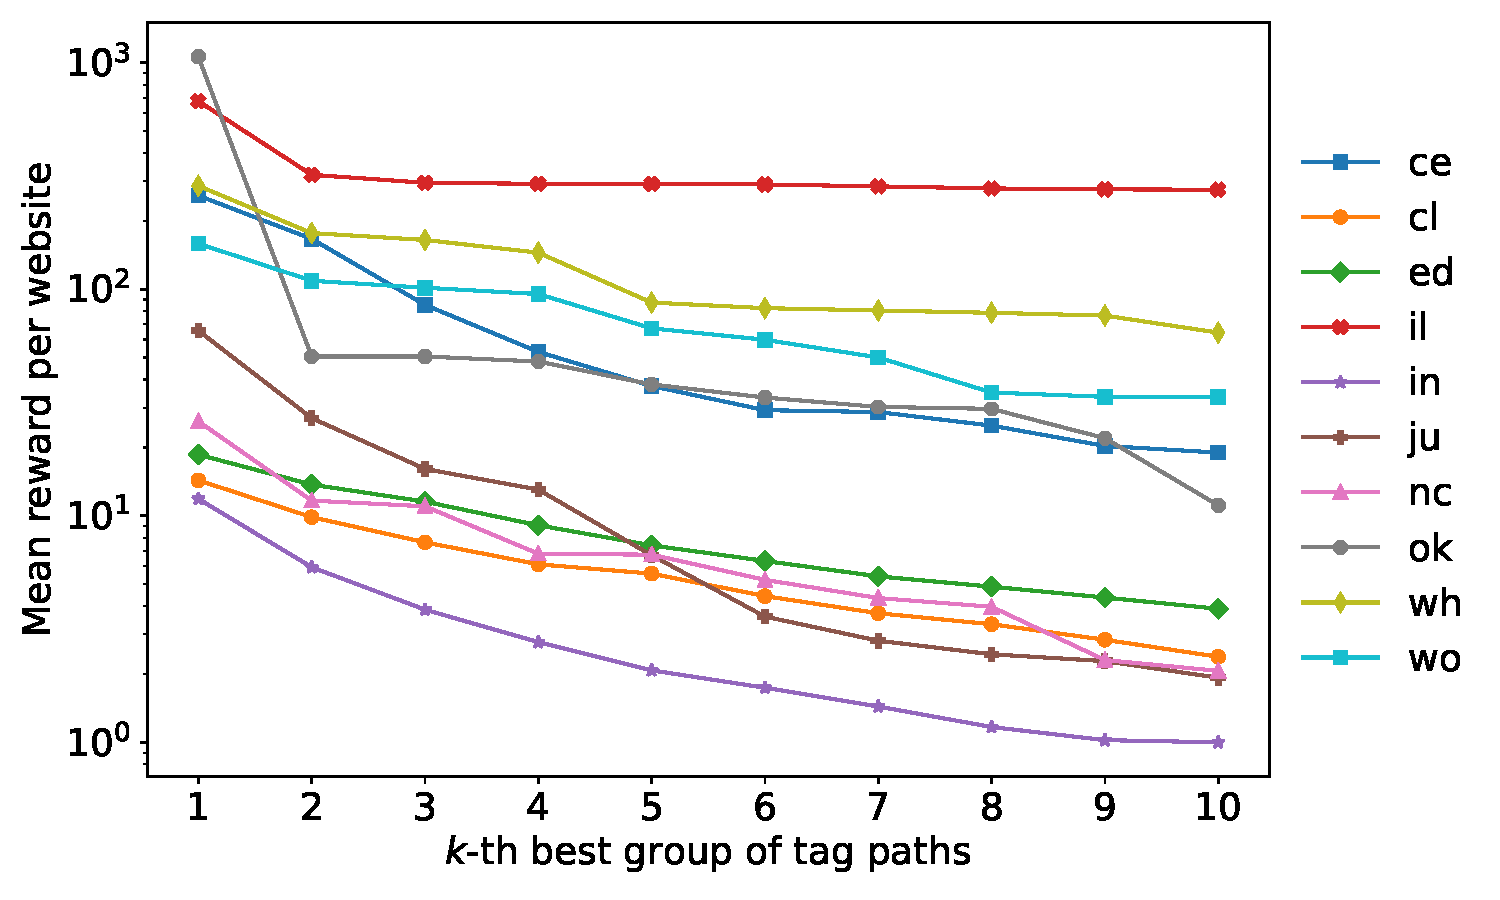
\includegraphics[width=\linewidth]{plots/top_k_dom_groups.pdf}
	\caption{Mean rewards of the top-10 groups of tag paths for the ten
  selected websites from Figure~\ref{fig:10_sites_plots} (log $y$-scale)}
	\label{fig:top_k_dom_groups}
\end{figure}

\begin{table*}
	\centering
	\caption{Mean and STD of non-zero rewards of the
  learning agent on each website}
	\begin{tabular}{ccccccccccccccccccc}
		\toprule
		               & \emph{ab} & \emph{as} & \emph{be} & \emph{ce} & \emph{cl} & \emph{cn} & \emph{ed} & \emph{il} & \emph{in} & \emph{is} & \emph{jp} & \emph{ju} & \emph{nc} & \emph{oe} & \emph{ok} & \emph{qa} & \emph{wh} & \emph{wo} \\
		\midrule
		\bfseries Mean & \01.7     & 1.5       & \04.5     & \030.2    & 12.4      & 4.2       & 2.5       & \03.1     & 1.6       & \03.5     & \03.5     & \05.4     & \02.0     & \02.5     & \05.5     & 15.4      & \03.0     & \02.1     \\
		\bfseries Std  & 16.8      & 5.35      & 20.9      & 290.3     & \02.8     & 8.9       & 7.1       & 53.9      & 4.2       & 11.1      & 17.4      & 10.5      & \08.7     & \09.3     & 13.9      & 18.8      & 22.0      & 43.5      \\
		\bottomrule
	\end{tabular}
	\label{tab:websites_rewards}
\end{table*}

We first study the reward associated by our algorithm to tag paths.
Figure~\ref{fig:top_k_dom_groups} shows the mean reward of the top 10
path groups (logarithmic $y$-axis), for the ten websites in Figure~\ref{fig:10_sites_plots}.
Top groups have high rewards: across websites, the best group averages 258, followed by 89, 74, 67, and 41 for the 10th, showing that \textbf{our SB agent effectively identifies tag path groups leading to HTML pages with target links}. Although the first group often dominates, several groups still yield substantial reward, so restricting to the top one is insufficient. Comparing Figure~\ref{fig:top_k_dom_groups} with the
mean rewards for each website (on groups with non-zero rewards)
in Table~\ref{tab:websites_rewards}, the top 10 groups
generally far exceed the overall mean
(e.g., for \emph{wo}, the the 10th group scores 33.5 v.s.\
 2.1 for the mean). This is also clear
from the high STD values from Table~\ref{tab:websites_rewards} (over 20 times the mean for \emph{wo})
implying significant differences in the rewards of different
	groups: rewards are not normally distributed across groups but more
closely resemble a power law.
Table~\ref{tab:websites_rewards} also shows large cross-website reward disparities, leading to the impossibility of setting an optimal exploration--exploitation trade-off coefficient~$\alpha$. This supports our pragmatic choice of $\alpha=2\sqrt{2}$, effective in practice. These disparities further highlight strong heterogeneity in target concentration across websites, complementing Sec.~\ref{subsection:dataset_characteristics}.

Examining top-group tag paths often reveals clues about target-rich areas. In \emph{nc}, a typical path includes \texttt{div.container.w-iap/}
\noindent\texttt{div.iap-content}, linked to the \emph{International Activities Program}, a program focused on collecting international education statistics. In \emph{wo}, paths include \texttt{collections-sief}, related to the \emph{Strategic Impact Evaluation Fund}, a trust fund producing data and reports. Some groups directly include target-retrieval keywords, e.g., \texttt{fr-link--download} in \emph{ju} or \texttt{status-publish} in \emph{ok}. Other websites' top paths are not  human-interpretable yet still achieve high rewards (examples in~\cite{github_repository}). This shows that our agent detects useful patterns even without semantic meaning, adapting to diverse structures without prior knowledge and supporting an online, per-website learning approach. 
It further demonstrates how our approach is language-independent: the RL agent learns structural patterns in HTML pages regardless of semantic meaning, enabling efficient target retrieval even on non-English or multilingual websites.

Assessing the concrete precision of our approach to retrieving SDs
requires determining the number of SDs collected in the targets.
Detecting statistics tables in heterogeneous formats is costly: even
state-of-the-art methods require roughly one second per PDF
page~\cite{soric2025benchmarkingtableextractionheterogeneous};
spreadsheets pose similar challenges~\cite{vitagliano2021detecting}.
Performing this online or at scale remains an open problem. As an empirical peak into the SD retrieval precision, we manually analyze a random sample of $7\times 40=280$ targets from 7 diverse websites in Table~\ref{tab:stats_tables}, counting the percentage of targets containing at least one statistics table (\textbf{``SD Yield''}) and their mean number per target (\textbf{``Mean \# SDs / Target''}). Results show that even on non-statistical websites (\emph{ed}, \emph{in}, \emph{oe}, \emph{wh}), an important fraction of targets contains SDs; although many targets contain none, SDs concentrate on a subset, yielding in most cases more than two SDs per collected target.

\begin{table}
	\centering
	\caption{SDs retrieval across sample targets}
	\begin{tabular}{lccccccc}
		\toprule
		& \emph{be} & \emph{ed} & \emph{is} & \emph{in} & \emph{nc} & \emph{oe} & \emph{wh} \\
		\midrule
		\bfseries SD Yield (\%) & 82 & 35 & 93 & 40 & 83 & 60 & 40 \\
		\bfseries Mean \# SDs / Target & 9.1 & 2.8 & 2.9 & 2.1 & 2.1 & 4.9 & 1.4 \\
		\bottomrule
	\end{tabular}
	\label{tab:stats_tables}
\end{table}

\begin{toappendix}
  \subsection{Effectiveness of SB Learning}

  A typical tag path containing reference to IAP in the website \emph{nc}
  is:
  \begin{quote}
    \path{/html/body/div.nces/div.container.w-iap/div.iap-content/div.row/div.col-md-6/h4/a}
  \end{quote}
  and to SIEF in the website \emph{wo}:
  \begin{quote}
  \path{/html/body/div.wp-page-body.container.default-wrapper page-collections.collections-sief/div.body-content-wrap.theme-nada-2/div.about-collection/div.repository-container/div.body/div/p/a}
  \end{quote}

  Examples of tag paths including keywords related to target retrieval are
  \begin{quote}
  \path{/html/body.path-node.page-node-type-ressource/div.dialog-off-canvas-main-canvas/div.layout-container/main#main-content/div.layout-content/div.region.region-content/div.block.block-system.block-system-main-block#block-open-theme-contenudelapageprincipale/article.mj-resource.mj-break-word.node--promoted/div.fr-container.mj-ressource__content/div.fr-grid-row.fr-grid-row--gutters.mj-content__corps/div.fr-col-lg-8.fr-col-offset-lg-2.fr-col-12.content-container__paragraph/section.fr-downloads-group.fr-downloads-group--multiple-links/ul/li/a.fr-link fr-link--download}
  \end{quote}
for \emph{ju}, and
  \begin{quote}
  \path{/html/body.home.page-template.page-template-onecolumn-page.page-template-onecolumn-page-php.page.page-id-7/main.content/div.container/div.row/div.main col-md-12/article.post.post-7.page.type-page.status-publish.hentry#post-7/div.entry-content/div#stcpDiv/div/strong/a}
  \end{quote}
for \emph{ok}.

Many other websites however have typical target-rich tag paths that cannot be interpreted by humans: for instance on \emph{jp} we have
  \begin{quote}
  \path{/html/body.top/div#wrapper/div#groval_navi/ul#groval_menu/li.menu-item-has-children/ul.sub-menu/li/a}
  \end{quote}
 on \emph{il} we have
  \begin{quote}
  \path{/html/body/div.container.s-lib-side-borders.pad-top-med#s-lg-side-nav-content/div.row/div.col-md-9/div.s-lg-tab-content/div.tab-pane.active#s-lg-guide-main/div.row.s-lg-row/div.col-md-12#s-lg-col-1/div.s-lg-col-boxes/div.s-lg-box-wrapper-17054143#s-lg-box-wrapper-17054143/div.s-lib-box-container#s-lg-box-14451639-container/div.s-lib-box.s-lib-box-std#s-lg-box-14451639/div#s-lg-box-collapse-14451639/div.s-lib-box-content/div.clearfix#s-lg-content-31285074/ul/li/a}
  \end{quote}
 and on \emph{ed} we have
  \begin{quote}
  \path{/html/body.cf-rtm/div.accueil-portail#page/div.container#main-ermes-container/main#main/div#readspeaker-container/div#portal/div.row/div.col-md-12.cms-inner-layout#layout-2/div.row/div.col-md-6.cms-inner-zone#zone-4/div#frame-224/div.frame.frame-portalcarouselwebframefactory.hidden-print/div.frame-standard.panel.panel-front.webframe-ermes-carousel/div.panel-body/div.ermes-frame-html#carousel-4AD04CE72B556A3CCF5DFCF7FB70964E/div.rsItem/div.modele_13.model-html/table/tbody/tr/td/a.vide}
  \end{quote}

\end{toappendix}

\begin{toappendix}
\subsection{URL Classification Quality}\label{subsubsection:url_classifier_results}

\begin{table}[h]
	\centering
  \vspace{-1em}
	\caption{Confusion matrix of the URL classifier, on the 11
		fully-crawled websites (average over 15 runs)}
	\vspace*{-.5em}
	\begin{tabular}{lrrr}
		\toprule
    \bfseries \diagbox{True}{Predicted} & \bfseries HTML (\%)    &
		\bfseries Target (\%)    & \bfseries Neither (\%)              \\
		\midrule
		\bfseries HTML           & 58.04                  & \01.37 & 0.00 \\
		\bfseries Target         & \00.75                 & 32.19  & 0.00 \\
		\bfseries Neither        & \05.34                 & \02.41 & 0.00 \\
		\bottomrule
	\end{tabular}
	\label{tab:cm_pcts_11_sites}
\end{table}

The confusion matrix of our URL classifier, averaged over 15 runs, for all fully-crawled websites, is presented
in Table~\ref{tab:cm_pcts_11_sites}.

We observe that classification errors are extremely marginal on ``HTML''
	and ``Target'' URLs. Never classifying as ``Neither'' leads to some
classification errors (discussed in Sec.~\ref{subsection:url_classifier}),
ultimately responsible for the difference between the number of requests 
made by
\textsf{\small SB-CLASSIFIER} and \textsf{\small SB-ORACLE} on the 11 fully-crawled websites. However, since the classifier oracle is unfeasible in
practice, the performance of
\textsf{\small SB-CLASSIFIER} is satisfactory.
\end{toappendix}

\subsection{Early-Stopping}\label{sec:early_stopping}

To prevent the crawler from continuing on websites with few or no remaining targets, we add an early-stopping mechanism. Every $\nu$ iterations, we compute a slope $\sigma = \tfrac{y_t - y_{t-\nu}}{\nu}$, representing the growth rate in the number $y_t$ of targets at crawling step~$t$. We then maintain an exponential moving average $\mu = \gamma \cdot \sigma + (1-\gamma)\cdot \mu$, with $\gamma$ the decay rate. If $\mu$ stays below a threshold $\epsilon$ for $\kappa$ consecutive slopes (i.e., $\kappa \cdot \nu$ iterations), crawling stops. Parameters ($\nu=1000$, $\epsilon=0.2$, $\gamma=0.05$, $\kappa=15$) provide a good balance between avoiding premature termination and efficiently stopping on exhausted sites.

The lower part of Table~\ref{tab:all_crawlers_all_sites_nb_requests} (below the double rule) shows early-stopping results: the percentage of requests avoided and of targets missed. High values are better for the former, low for the latter. We observe three behaviors:
\begin{inparaenum}[(i)]
  \item Medium to large websites where target discovery slows and stopping occurs effectively (\emph{ab}, \emph{ed}, \emph{in}, \emph{jp}, \emph{ju}, \emph{nc}, \emph{ok}). Smaller sites take longer (in \%) to stop due to the required $\kappa \cdot \nu$ iterations;
  \item Large websites with continuous target discovery where stopping conditions are never met before manual termination (\emph{as}, \emph{ce}, \emph{il}, \emph{oe}, \emph{wh}, \emph{wo});
	\item Small sites (\emph{be}, \emph{cl}, \emph{cn}, \emph{qa}) where the crawl ends before early stopping can trigger within $\kappa \cdot \nu = 15$k iterations; this is not an issue, as these sites are quickly fully crawled.
\end{inparaenum}

\begin{toappendix}
  \subsection{Early-Stopping}
  \begin{figure}[h]
	\begin{subfigure}[t]{0.49\linewidth}
		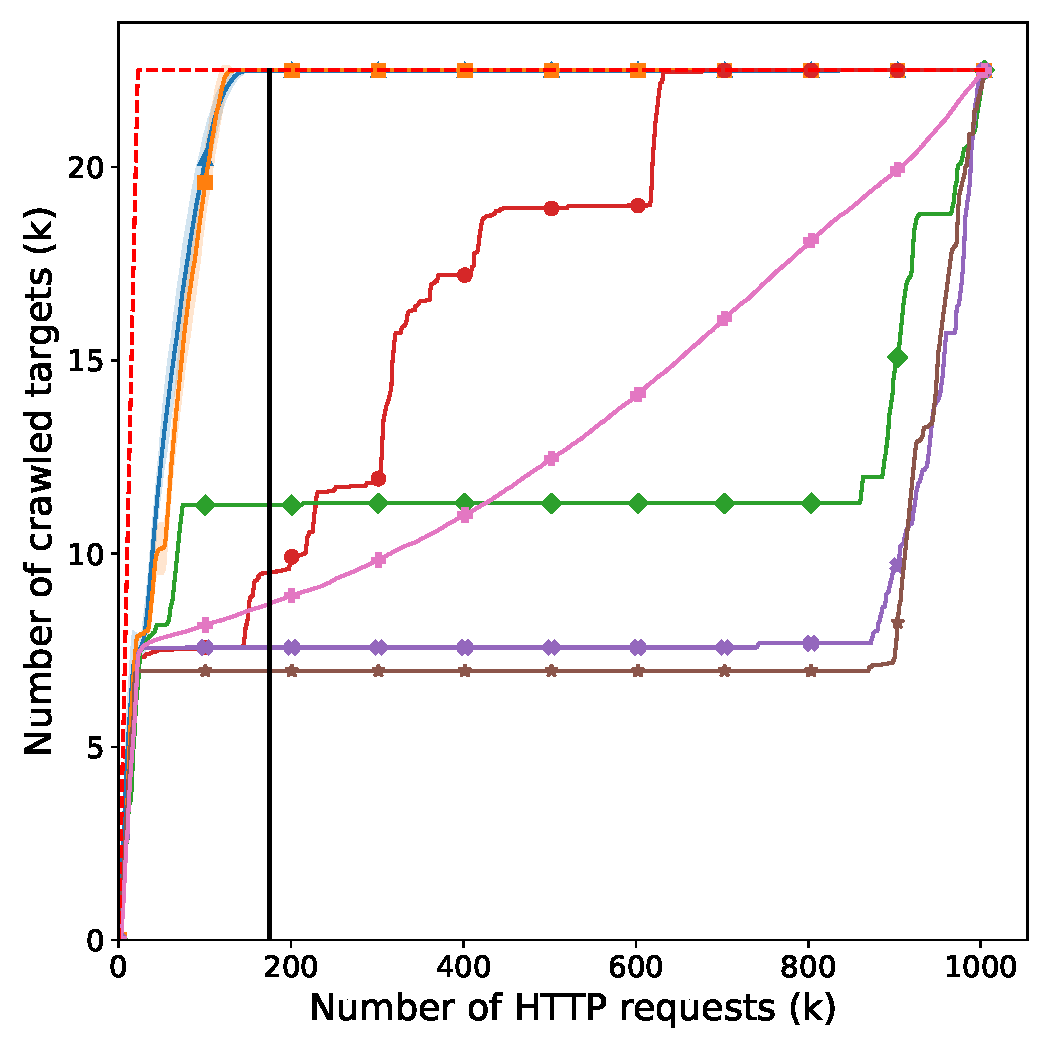
\includegraphics[width=\linewidth]{plots/early_stopping/in.pdf}

		\vspace{-1em}
		\caption{\emph{in}}
		\label{fig:in_early_stopping}
	\end{subfigure}
	\begin{subfigure}[t]{0.49\linewidth}
		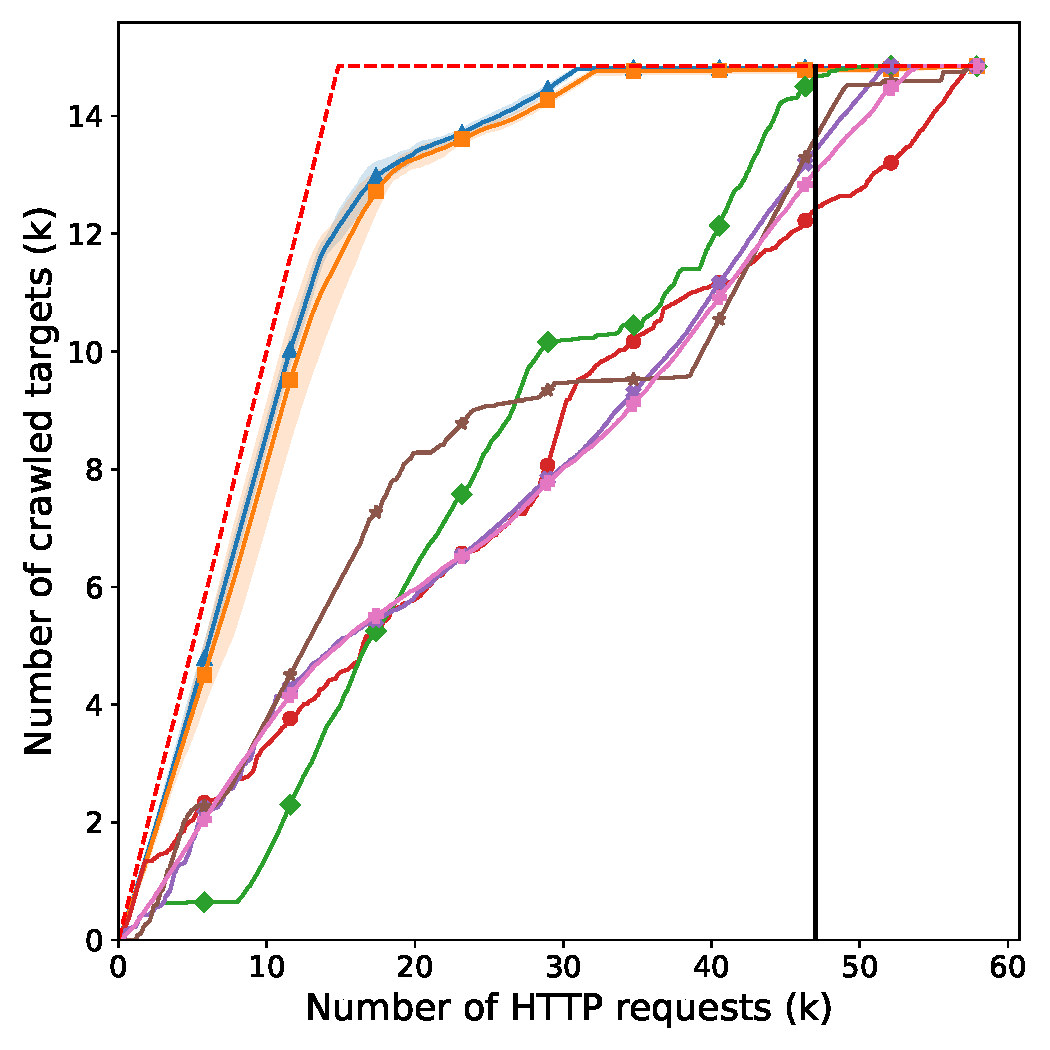
\includegraphics[width=\linewidth]{plots/early_stopping/ju.pdf}

		\vspace{-1em}
		\caption{\emph{ju}}
		\label{fig:ju_early_stopping}
	\end{subfigure}
	\vspace{-.75em}
	\caption{Visualization of early-stopping time (black rule) for websites \emph{in} and \emph{ju}}
	\label{fig:early_stopping_in_ju}
\end{figure}

	Figure~\ref{fig:early_stopping_in_ju} presents a visualization of
  the early-stopping mechanism applied to two websites: \emph{in} and
\emph{ju} (right). Both fall under the first behavior described in
Sec.~\ref{sec:early_stopping}, illustrating that smaller websites take
longer (in \%) to stop after the first signs of target convergence. For
\emph{in}, stopping occurs shortly after the point where a human would
likely have cut, but for \emph{ju}, the delay is more important. Despite
early signs of convergence, stopping is postponed due to the fixed
$\kappa \cdot \nu =15\,000$ threshold, which represents a much larger fraction of the site for \emph{ju} (60k pages) than for \emph{in} (1M pages).

\bigskip
\end{toappendix}

\begin{comment}
\begin{table}
	\centering
	\caption{Confusion matrix of the URL classifier used in the SB algorithm on website \emph{be} (on average, for 15 runs).}
	\begin{tabular}{lrrr}
		\toprule
		\bfseries True/Predicted & \bfseries HTML & \bfseries Target & \bfseries Neither \\
		\midrule
		\bfseries HTML           & 11231          & \0\0272          & \0\0\0\00         \\
		\bfseries Target         & \0\0732        & 15321            & \0\0\0\00         \\
		\bfseries Neither        & \02436         & \02296           & \0\0\0\00         \\
		\bottomrule
	\end{tabular}
	\label{tab:cm_be}
\end{table}

% 34.784  0.842 0
% 2.267 47.451 0
% 7.545 7.111 0

\begin{table}
	\centering
	\caption{Confusion matrix of the URL classifier used in the SB algorithm on website \emph{cl} (on average, for 15 runs).}
	\begin{tabular}{lrrr}
		\toprule
		\bfseries True/Predicted & \bfseries HTML & \bfseries Target & \bfseries Neither \\
		\midrule
		\bfseries HTML           & 1654           & \0\024           & \0\0\00           \\
		\bfseries Target         & \0154          & 3538             & \0\0\00           \\
		\bfseries Neither        & \0104          & \0340            & \0\0\00           \\
		\bottomrule
	\end{tabular}
	\label{tab:cm_cl}
\end{table}

% 28.449 4.128 0
% 2.649 60.853 0
% 3.696  5.848 0

\begin{table}
	\centering
	\caption{Confusion matrix of the URL classifier used in the SB algorithm on website \emph{cn} (on average, for 15 runs).}
	\begin{tabular}{lrrr}
		\toprule
		\bfseries True/Predicted & \bfseries HTML & \bfseries Target & \bfseries Neither \\
		\midrule
		\bfseries HTML           & 5272           & \0\0\07          & \0\0\00           \\
		\bfseries Target         & \0\064         & 7423             & \0\0\00           \\
		\bfseries Neither        & \0\0\08        & \0\016           & \0\0\00           \\
		\bottomrule
	\end{tabular}
	\label{tab:cm_cn}
\end{table}

% 41.220 0.055 0
% 0.500 58.038 0
% 0.063 0.125 0

\begin{table}
	\centering
	\caption{Confusion matrix of the URL classifier used in the SB algorithm on website \emph{ed} (on average, for 15 runs).}
	\begin{tabular}{lrrr}
		\toprule
		\bfseries True/Predicted & \bfseries HTML & \bfseries Target & \bfseries Neither \\
		\midrule
		\bfseries HTML           & 85920          & \02610           & \0\0\0\0\00       \\
		\bfseries Target         & \0\0175        & 10180            & \0\0\0\0\00       \\
		\bfseries Neither        & \08645         & \01348           & \0\0\0\0\00       \\
		\bottomrule
	\end{tabular}
	\label{tab:cm_ed}
\end{table}

% 78.914 2.397 0
% 0.160 9.350 0
% 7.940 1.238 0

\begin{table}
	\centering
	\caption{Confusion matrix of the URL classifier used in the SB algorithm on website \emph{in} (on average, for 15 runs).}
	\begin{tabular}{lrrr}
		\toprule
		\bfseries True/Predicted & \bfseries HTML & \bfseries Target & \bfseries Neither \\
		\midrule
		\bfseries HTML           & 883706         & \0\0\0164        & \0\0\0\0\00       \\
		\bfseries Target         & \0\0\0117      & \022362          & \0\0\0\0\00       \\
		\bfseries Neither        & \092544        & \0\03922         & \0\0\0\0\00       \\
		\bottomrule
	\end{tabular}
	\label{tab:cm_in}
\end{table}

% 88.123 0.016 0
% 0.012 2.230 0
% 9.228 0.391 0

\begin{table}
	\centering
	\caption{Confusion matrix of the URL classifier used in the SB algorithm on website \emph{is} (on average, for 15 runs).}
	\begin{tabular}{lrrr}
		\toprule
		\bfseries True/Predicted & \bfseries HTML & \bfseries Target & \bfseries Neither \\
		\midrule
		\bfseries HTML           & 118805         & \0\0\0113        & \0\0\0\0\00       \\
		\bfseries Target         & \0\0\0120      & 168762           & \0\0\0\0\00       \\
		\bfseries Neither        & \0\01185       & \0\02292         & \0\0\0\0\00       \\
		\bottomrule
	\end{tabular}
	\label{tab:cm_is}
\end{table}

% 40.788 0.039 0
% 0.041 57.939 0
% 0.407 0.787 0

\begin{table}
	\centering
	\caption{Confusion matrix of the URL classifier used in the SB algorithm on website \emph{ju} (on average, for 15 runs).}
	\vspace{-.5em}
	\begin{tabular}{lrrr}
		\toprule
		\bfseries True/Predicted & \bfseries HTML & \bfseries Target & \bfseries Neither \\
		\midrule
		\bfseries HTML           & 40657          & \0\0143          & \0\0\0\0\00       \\
		\bfseries Target         & \0\0134        & 14711            & \0\0\0\0\00       \\
		\bfseries Neither        & \0\0404        & \01045           & \0\0\0\0\00       \\
		\bottomrule
	\end{tabular}
	\label{tab:cm_ju}
\end{table}

% 71.211 0.250 0
% 0.235 25.676 0
% 0.708 1.830 0

\begin{table}
	\centering
	\caption{Confusion matrix of the URL classifier used in the SB algorithm on website \emph{nc} (on average, for 15 runs).}
	\vspace{-.5em}
	\begin{tabular}{lrrr}
		\toprule
		\bfseries True/Predicted & \bfseries HTML & \bfseries Target & \bfseries Neither \\
		\midrule
		\bfseries HTML           & 217531         & \02193           & \0\0\0\0\00       \\
		\bfseries Target         & \0\0\0839      & 82187            & \0\0\0\0\00       \\
		\bfseries Neither        & \0\03033       & \01222           & \0\0\0\0\00       \\
		\bottomrule
	\end{tabular}
	\label{tab:cm_nc}
\end{table}

% 70.856 0.714 0
% 0.273 26.771 0
% 0.988 0.398 0

\begin{table}
	\centering
	\caption{Confusion matrix of the URL classifier used in the SB algorithm on website \emph{oe} (on average, for 15 runs).}
	\vspace{-.5em}
	\begin{tabular}{lrrr}
		\toprule
		\bfseries True/Predicted & \bfseries HTML & \bfseries Target & \bfseries Neither \\
		\midrule
		\bfseries HTML           & 143412         & 11071            & \0\0\0\0\00       \\
		\bfseries Target         & \0\01046       & 42150            & \0\0\0\0\00       \\
		\bfseries Neither        & \0\03427       & \09994           & \0\0\0\0\00       \\
		\bottomrule
	\end{tabular}
	\label{tab:cm_oe}
\end{table}

% 67.936 5.244 0
% 0.495  19.967 0
% 1.623 4.734 0

\begin{table}
	\centering
	\caption{Confusion matrix of the URL classifier used in the SB algorithm on website \emph{ok} (on average, for 15 runs).}
	\vspace{-.5em}
	\begin{tabular}{lrrr}
		\toprule
		\bfseries True/Predicted & \bfseries HTML & \bfseries Target & \bfseries Neither \\
		\midrule
		\bfseries HTML           & 391802         & \03556           & \0\0\0\0\00       \\
		\bfseries Target         & \0\0\0669      & 12058            & \0\0\0\0\00       \\
		\bfseries Neither        & \012484        & \02206           & \0\0\0\0\00       \\
		\bottomrule
	\end{tabular}
	\label{tab:cm_ok}
\end{table}

% 422775
% 92.674 0.841 0
% 0.158  2.852 0
% 2.953 0.522 0

\begin{table}
	\centering
	\caption{Confusion matrix of the URL classifier used in the SB algorithm on website \emph{qa} (on average, for 15 runs).}
	\begin{tabular}{lrrr}
		\toprule
		\bfseries True/Predicted & \bfseries HTML & \bfseries Target & \bfseries Neither \\
		\midrule
		\bfseries HTML           & 1311           & \0\031           & \0\0\00           \\
		\bfseries Target         & \0\077         & 2356             & \0\0\00           \\
		\bfseries Neither        & 1320           & \0247            & \0\0\00           \\
		\bottomrule
	\end{tabular}
	\label{tab:cm_qa}
\end{table}

% 24.541 0.580 0
% 1.441 44.103 0
% 24.71 4.624 0
\end{comment}
